\section{Materials and Methods}
    
    \subsection{Measurement Set-up}
    
        The experimental set-up consisted of a single strawberry plant (\textit{Fragaria $\times$ ananassa}), placed inside a growth chamber of \SI[product-units = single]{1.45 x 0.77 x 1.45}{\metre} (height $\times$ depth $\times$ width) (BIOCLIM 1600 US, Weiss Technik, Reiskirchen, Germany). Light intensity, temperature and relative humidity were controlled by a microcontroller board (Dwenguino, Dwengo~vzw, Brussels, Belgium), placed outside the growth chamber. The temperature and relative humidity of the growth chamber were controlled using analogue signals, and varied randomly between \SIlist{11;33}{\celsius}, and  \SIlist{31;75}{\percent} respectively.
        
        A custom-built frame of \SI[product-units = single]{1.00 x 0.70 x 1.10}{\metre} (height $\times$ depth $\times$ width) was inserted into the chamber. On top of which a grid of lamps was mounted, consisting of 32~LED lamps (MAS LED spot VLE D 4.9-50W GU10 927 60D, Koninklijke Philips N.V., Amsterdam, The Netherlands) and twelve halogen lights (DECOSTAR 51 PRO 50 W 12 V \ang{36} GU5.3, OSRAM GmbH, Munich, Germany). The halogen lights were used as broadband light source, providing illumination in the visible and infrared range, while the LED lights increased the total Photosynthetically Active Radiation (PAR) while keeping thermal radiation within limits. The light intensity of the halogen lamps was controlled using a Digital Addressable Lighting Interface (DALI) controller and bus, while the LED lights were arranged in four sets that could be individually turned on and off. A detailed overview of the grid is depicted in \cref{lamp-configuration}.
        
        \begin{figure}[thb]
            \centering
            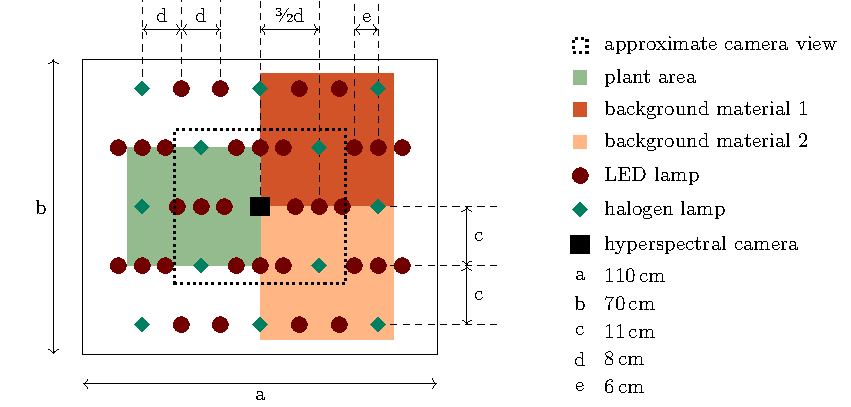
\includegraphics{figures/lamp-layout}
            \caption{Schematic representation of the light and camera arrangement above the plant and background materials.}
            \label{lamp-configuration}
        \end{figure}
        
        A single strawberry leaf was inserted into a transparent leaf chamber of the LI-6400XT photosynthesis system (LI-COR, Lincoln, NE, USA) to acquire gas exchange measurements (transpiration and photosynthesis). The control board also controlled the sampling time steps of the LI-6400XT, using a custom circuit that was connected to the manual sample button on the measurement node. To increase the carbon dioxide concentration in the growth chamber, a constant influx of stabilised air was used. This influx had a carbon dioxide concentration of \SI{500}{ppm} at a rate of \SI{1}{\cubic\metre \per\hour}. For environment sensing at canopy height, we measured the temperature, light intensity and relative humidity. An external probe (Vaisala 50Y, Vaisala, Helsinki, Finland) was used to measure temperature and humidity. The gas exchange device has a PAR probe to measure light intensity. This device was programmed to recreate the temperature measured using the probe inside the chamber, thus preventing the chamber from heating-up due to infrared radiation.
        
        In the centre of the lamp grid, a hyperspectral camera consisting of two camera heads (EP-12, {3D-One}, Sulz, Austria) was placed to monitor the plant. One head is sensitive light in the near-infrared (NIR), while the other is sensitive to the visible range (VIS). We refer to these as H1 and H2, respectively. Both heads capture \SI{12}{\bit} colour information. The sensors were constructed by IMEC (Leuven, Belgium).
        H1 captures light in 25~spectral bands and has a spatial resolution of $403 \times 216$. H2 captures light in 16~spectral bands and has a spatial resolution of $504 \times 270$. A trade-off was made here between spectral accuracy and sampling rate. We set the sampling period to \SI{3}{\second}, which was too fast for using a high-resolution line-scanning sensor. The snapshot camera used here can capture images up to \SI{120}{\hertz}. 
        One spectral filter was used for each sensor to limit the sensitivity range of the visible (VIS) or near-infrared (NIR) spectra. The NIR filter was a long pass filter, starting at \SI{675}{\nano\metre} and cuts-off at \SI{1650}{\nano\metre} (TECHSPEC 675nm 25mm Dia, High Performance Longpass Filter, Edmund Optics, Barrington, NJ, USA), while the VIS filter (SCHOTT BG38, Edmund Optics, Barrington, NJ, USA) starts at \SI{350}{\nano\metre} and cuts-off at \SI{645}{\nano\metre}. This camera does not support an external trigger source, thus the internal trigger source was configured to sample every \SI{3}{\second}. When the responses of the cameras were taken into account, this set-up observed wavelengths in the ranges \SIrange{400}{645}{\nano\metre}, and \SIrange{675}{1000}{\nano\metre} for H1 and H2 respectively. %The detectors are not sensitive to light above \SI{1000}{\nano\metre}. 
        An illustration of the entire set-up is shown in \cref{setup-overview}.
        
        \begin{figure}[thb]
            \centering
            \includegraphics{figures/setup-overview}
            \caption{Experimental set-up inside the growth chamber. The plant (strawberry) was raised to increase the area of the leaf in the images. The sensors (photodiodes, relative humidity and temperature sensor) were mounted at canopy height. The hyperspectral camera was mounted directly above the plant. Twelve halogen lights were mounted at the same height as the camera. A grey PVC plate was used to provide a uniform background.}
            \label{setup-overview}
        \end{figure}
        
        The spectral resolution of H1 varies between \SIlist{6;25}{\nano\metre}, while the spectral resolution of H2 varies between \SIlist{2;14}{\nano\metre}.
        
        A camera always makes an indirect observation, so there might be unwanted interference with the measurements. For instance, the reflective properties of surrounding materials can change, which interferes with the plant measurements. To investigate this, we also included different background materials in the analysis. Four materials were investigated: plywood (hardwood, Van Den Nest, Aalst, Belgium), non-reflective black cotton cloth (Veritas, Kontich, Belgium), grey polyvinyl chloride (PVC) (Scafoam, Scala, Wetteren, Belgium), and Ytong (Xella, Duisburg, Germany). It was not possible to have similar lighting conditions on all four materials simultaneously. Consequently, the experiment was conducted twice. The first experiment used PVC and plywood, while the second used Ytong and cloth. The second experiment was conducted four days after the first one on a different plant. Both plants were grown in the same greenhouse in close proximity, and thus experienced similar conditions before the experiment. Each experiment lasted for \SI{100}{\hour}. Temperature, relative humidity and light radiation were randomly varied, but the same time series was used in both experiments. To generate these random sequences, samples were drawn from a uniform distribution. These distributions ranged between 
        \SIrange{8.8}{32.6}{\celsius} and \SIrange{38.8}{94.6}{\percent} for temperature and relative humidity respectively. These are the set values, which differ from the measured values mentioned above, because the growth chamber was not always able to respond sufficiently fast to the target conditions. The halogen lights were controlled digitally using the DALI interface with brightness vales between 196 (0xC4) and 254 (0xFE) (the maximum value), while the four sets of LED lights were set by sampling a number between 0 and 15, where each bit corresponds to the status of a lamp set. 
        
        \begin{alignat}{2}
            VI^{F}_{ij} &= \dfrac{C_i}{C_j},            &\quad&i \in\{0,1,\ldots,40\}, j \in \{0,1,\ldots,i-1,i+1,\ldots,40\} \label{vi1} \\
            VI^{NF}_{ij} &= \dfrac{C_i - C_j}{C_i+C_j}, &&i \in\{0,1,\ldots,39\}, j \in \{i+1, i+2, \ldots,40\} \label{vi2}
        \end{alignat}
        
        Normally, VIs are only generated on image data from plants, but we also generated them for the background materials to avoid bias due to the generation of possibly more informative features in the comparison between plant- and background-based models.
        
        To assess the variability in performance due to the subsampling in the second dataset, nine independent subsets were constructed of each subsample size. Consequently, partial overlap between datasets was possible.
        
        A linear model combined with Tikhonov (or L2) regularisation \citep{tikhonovSolution1963}, commonly called ridge regression, was used to fit the camera data to the environmental and eco-physiological data. Such a model is well-suited to demonstrate correlations between different datasets and should provide improved prediction performance compared to only using indices \citep{yendrekHighThroughput2017}. It is guaranteed to provide the global optimum and is very fast to fit. This is important since hyperspectral cameras generate vast amounts of data. The Tikhonov regularisation prevents the model to overfit by including the model weights into the optimisation target. 
        The whole pipeline was implemented in Python, with the help of the Pandas \citep{mckinneyData2010,mckinneyPandas2011} and Scikit-Learn \citep{pedregosaScikitlearn2011} libraries and has been open-sourced on GitHub\footnote{\url{https://github.com/opieters/hyperspectral-analysis}}. Part of the dataset is also available with an open-access licence on Zenodo \citep{pieters2020}.
        
        Ridge regression has one hyperparameter that must be optimised. This parameter determines the total magnitude of the model coefficients. As a result, each time series had to be split into three categories: training, validation and test data. The training data was used to train the coefficients of the model, while the validation data was used to select the optimal hyperparameter. The test data was employed to evaluate the performance on unseen data. This latter type of data was not used to optimise the model in any way and thus provided a good indication for the actual performance of the model. To eliminate possible day-night rhythms, the data was split into batches of 3000~samples (\SI{2.5}{\hour}), while 1500~samples (\SI{1.25}{\hour}) between batches were discarded to eliminate the correlation between adjacent batches. This decorrelation was verified after the analysis through an offset between the target and input data (not shown). After selecting the optimal hyperparameter, a final model was trained on both the train and validation data.
        
        \begin{figure}[thb]
            \centering
            \includegraphics{figures/split-visualisation}            
            \caption{Visualisation of the data split in training, validation, and test data for both experiments.}
            \label{data-split}
        \end{figure}
        
        In summary, three different types of linear models were generated based on six different data types. The three model types refer to the kind of input features presented to the model. In the first case, the model was trained on the averaged spectral bands. In the second case, VIs were added to the input feature set. This data-augmentation enabled the model to leverage non-linear dependencies in the data. In the third and final case, the input features consisted entirely of spectral bands, but without averaging over the entire mask. Different materials give rise to distinct data types; plant1, plant2, wood, PVC, Ytong and cotton were the materials considered in this study.
        
    \subsection{Error Metric}
        
        To estimate the modelling capacity of the camera system, different models were created that estimate environmental and eco-physiological data. Comparing the performance of different tasks is crucial. To that end, the normalised mean squared error (NMSE) metric was used:
        
        \begin{equation}
          \text{NMSE} = \ddfrac{\frac{1}{N}\sum_{t=0}^{N-1} (y(t)-\hat{y}(t))^2}{\text{var}(y)} 
        \end{equation}
        
        where $\hat{y}(t)$ is the predicted value from the model, $y(t)$ is the actual value, $\text{var}(\cdot)$ computes the variance and $N$ is the total number of samples considered. This metric has several advantages over a traditional mean squared error comparison. In the first place, it takes the variability of the target signal into account. This eliminates a possible bias towards slow varying signals. Additionally, interpretability is very straightforward. An NMSE of 1.0 corresponds to the mean prediction for all samples, since the numerator reduces to the variance, while an NSME of 0.0 corresponds to a perfect prediction. This property makes it very easy to compare and interpret NMSE values.
        
    \subsection{Variables and Eco-physiological Meaning}  
    
        The gas exchange measurement device (LI6400XT) produced the eco-physiological data to which the hyperspectral image data was fitted. Different environmental and eco-physiological parameters were captured, providing a diverse set of target variables. An overview of the available variables is provided in \cref{parameter-overview}. All variables except for air temperature (\Tair) and relative humidity (\RH) were measured outside the area observed with the camera. This was a requirement due to the high reflectivity of the leaf chamber that resulted in an undesired exposure compensation of the camera. 
        
        \begin{table}[thb]
            \centering
            \caption{Overview of considered environmental and eco-physiological variables.}
            \label{parameter-overview}
            \begin{tabular}{C{2.5cm}L{5cm}C{4cm}C{2.5cm}}
                \toprule
                \textbf{abbreviation} & \textbf{description} & \textbf{unit} & \textbf{sensor}\\
                \midrule
                \arrayrulecolor{black!10!white}
                \Photo & photosynthetic rate & 
                  \si{\micro\mole \of{CO\textsubscript{2}} \per\square\metre \per\second} &
                  LI6400XT \\ 
                \midrule
                \Cond & stomatal conductance & 
                  \si{\mole \of{H\textsubscript{2}O} \per\square\metre \per\second} &
                  LI6400XT \\
                \midrule
                \Transp & transpiration rate & 
                  \si{\milli\mole \of{H\textsubscript{2}O} \per\square\metre \per\second} &
                  LI6400XT \\
                \midrule
                \VPDL & vapour pressure deficit based on leaf temperature & 
                  \si{\kilo\pascal} & LI6400XT\\
                \midrule
                \Tleaf & leaf temperature & \si{\celsius} & LI6400XT \\
                \midrule
                \Tair & {air temperature\newline(growth chamber)} & \si{\celsius} & Vaisala 50Y \\
                \midrule
                \RH & {relative humidity\newline(growth chamber)} & \si{\percent} & Vaisala 50Y\\
                \midrule
                \PAR & {photosynthetically active radiation (growth chamber)} &    
                  \si{\micro\mole\per\square\metre\per\second} & LI6400XT \\
                \arrayrulecolor{black}
                \bottomrule
            \end{tabular}
        \end{table}